\documentclass[11pt]{article}
\usepackage{amsmath}
\usepackage{gensymb}
\usepackage{graphicx}
\usepackage{listings}
\usepackage{xcolor}
\usepackage[margin=1in]{geometry}

% Set up for code listing
\lstset{
    language=Matlab,
    basicstyle=\ttfamily\small,
    keywordstyle=\color{blue},
    commentstyle=\color{green},
    morecomment=[l][\color{magenta}]{\#},
    frame=single,
    breaklines=true
}

\begin{document}
\title{ELCT 331 Control Systems Assignment 5}
\author{Jacob C. Vaught}
\date{December 13th, 2023}
\maketitle

\section*{Problem 7-12 [45 points]}
Construct the Root Locus diagram for each of the following control systems for which the poles and zeros of \( G(s)H(s) \) are given. The characteristic equation is obtained by equating the numerator of \( 1 + G(s)H(s) \) to zero. Determine the Range of K that the system is stable in.

\begin{enumerate}
    \item Poles at \( 0, -1, -3, -4 \); no finite zeros
    \item Poles at \( 0, -1+j, -1-j \); zero at \( -2 \)
    \item Poles at \( 0, -1+j, -1-j \); no finite zeros
\end{enumerate}

\newpage
\subsection*{Solution for Problem part A}

\subsubsection*{Open-Loop Gain \( K(s) \) and its Derivative \( K'(s) \):}
The open-loop transfer function \( K(s) \) for a system with poles at \( 0, -1, -3, -4 \) and no zeros is given by:
\begin{align*}
    K(s) &= -s(s+1)(s+3)(s+4),
\end{align*}
The derivative \( K'(s) \) is calculated to find the breakaway points:
\begin{align*}
    K'(s) &= \frac{d}{ds}[-s(s+1)(s+3)(s+4)] \\
          &= -4s^3-24s^2-38s-12
\end{align*}

\subsubsection*{Finding Breakaway Points:}
The breakaway points occur where \( K'(s) = 0 \):
\begin{align*}
    0 &= -4s^3 - 24s^2 - 38s - 12, \\
    0 &= 4s^3 + 24s^2 + 38s + 12 \\
    s &= -2, -2 + 0.5\sqrt{10}, -2 - 0.5\sqrt{10} \\
    s &= -3.58, -2, -0.42
\end{align*}

\subsubsection*{Asymptotes:}
The angles (\(\phi\)) and centroids (\(\sigma\)) of the asymptotes are determined by:
\[\sigma = \frac{\text{Sum of real parts of poles - Sum of real parts of zeros}}{\text{Number of poles - Number of zeros}}\]
\[\phi = \frac{(2i+1)\pi}{\text{Number of poles - Number of zeros}}\]
\newline
For our system:
\[\sigma = \frac{0+(-1)+(-3)+(-4)}{4-0}=-2\]
\[\phi = \frac{(2i+1)\pi}{4-0} = 45\degree, 135\degree, 225\degree, 315\degree \text{ for } i=0,1,2,3.\]

\subsubsection*{Intersects with the Imaginary Axis:}
The intersection with the imaginary axis is found by analyzing the characteristic equation:
\[\frac{G}{1+GH} = \frac{G(s)}{1+\frac{K}{s(s+1)(s+3)(s+4)}}=\frac{s(s+1)(s+3)(s+4)G(s)}{s(s+1)(s+3)(s+4)+K}\]
\newline
The characteristic equation for stability analysis is given by setting the denominator of the closed-loop transfer function to zero:
\[1 + G(s)H(s) = 0 \Rightarrow \text{Characteristic Equation}\]
\newline
In our case, the characteristic equation is:
\[s^4+8s^3+19s^2+12s+K=0\]
\newline
For stability analysis, we substitute \( s=j\omega \) (where \( j \) is the imaginary unit) into the characteristic equation. This substitution separates the equation into its real and imaginary parts.
\newline
The imaginary part yields:
\[-8(j\omega)^3 + 12(j\omega) = 0\]
Simplifying the imaginary part, we get:
\[-8\omega^3+12\omega=0\]
From this equation, we find the values of \( \omega \) where the root locus crosses the imaginary axis:
\[\omega = 0, \pm\sqrt{\frac{12}{8}}\]
\newline
The real part of the equation becomes:
\[(j\omega)^4 + 8(j\omega)^3 + 19(j\omega)^2 + 12(j\omega) + K = 0\]
Simplifying the real part, we obtain:
\[\omega^4 - 19\omega^2 + K = 0\]
\newline
This equation is used to find the value of \( K \) for the given \( \omega \) from the previous section:
\[\omega^4 - 19\omega^2 + K = 0 \Rightarrow \omega = 0, \pm\sqrt{\frac{12}{8}}, \text{ and } K = 0, 26.1\]
\newline
The system will be unstable for \( K>26.1 \).

% Importing the root locus plot image
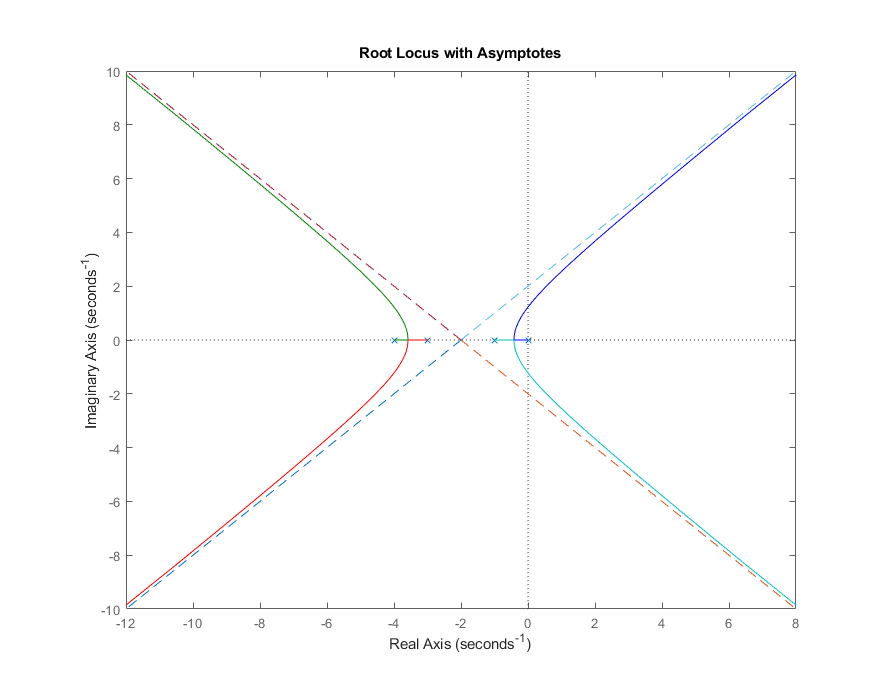
\includegraphics[width=0.8\textwidth]{7-12B_fig.png}


% MATLAB code listing
\begin{lstlisting}
poles = [0, -1, -3, -4]; % Poles of the system
G = tf(1, poly(poles)); % Transfer function G(s)

figure;
rlocus(G);
hold on;

num_poles = length(poles);
sigma = sum(poles) / num_poles; % Centroid of asymptotes
angles_rad = deg2rad((2*(0:num_poles-1) + 1) * 180 / num_poles);

% Plotting asymptotes
for angle = angles_rad
    far_point = sigma + 1000*exp(1i*angle); 
    % Draw the asymptote
    plot([sigma, real(far_point)], [0, imag(far_point)], '--');
end

title('Root Locus with Asymptotes');
xlabel('Real Axis');
ylabel('Imaginary Axis');
hold off;
\end{lstlisting}


\newpage
\subsection*{Solution for Problem part B}

\subsubsection*{Open-Loop Gain \( K(s) \) and its Derivative \( K'(s) \):}
The open-loop transfer function \( K(s) \) for a system with poles at \( 0, -1+j, -1-j \) and a zero at \( -2 \) is given by:
\begin{align*}
    K(s) &= \frac{K}{(s+2)(s+1-j)(s+1+j)}, \\
         &= \frac{K}{s(s^2+2s+2)}.
\end{align*}
This transfer function is derived by multiplying the factors corresponding to each pole and zero. The open-loop gain \( K \) is generally a variable representing the system gain.
\newline
\textbf{Root Locus on Real Axis:} The root locus exists on the real axis to the left of an odd number of poles and zeros. In this case, it's between \( 0 \) and \( -2 \).
\newline
\textbf{Breakaway Points:} Breakaway points are found by differentiating \( K(s) \) and equating to zero. However, in this system, there are no real-axis breakaway points because the derivative of \( K(s) \) does not yield any real roots within the range of the poles.

\subsubsection*{Asymptotes:}
The angles (\(\phi\)) and centroids (\(\sigma\)) of the asymptotes are determined by:
\[\sigma = \frac{\text{Sum of real parts of poles - Sum of real parts of zeros}}{\text{Number of poles - Number of zeros}} = \frac{(0+(-1)+(-1)) - (-2)}{3-1} = 0\]
\[\phi = \frac{(2i+1)\pi}{\text{Number of poles - Number of zeros}} = \pm 90^\circ \text{ for } i=0,1.\]
These calculations give the directions in which the root locus branches will approach infinity.
\newline
\textbf{Departure Angle Calculation:} Departure angles are calculated when the poles are complex. They determine the initial angle at which the root locus leaves a complex pole. The angle is calculated by summing the angles made with all other poles and zeros and subtracting from \( 180^\circ \).
\newline
In this case, the departure angle from the pole at \( -1-j \) is:
\[\theta_1 - (\theta_2 + \theta_3 + \theta) = 180^\circ\]
where \(\theta_1\) is the angle to the zero and \(\theta_2\) and \(\theta_3\) are the angles to the other two poles. The calculated angles give \(\theta = 0^\circ\).
\newline
\textbf{Stability Analysis:} Since the root locus is on the left half of the s-plane (real part of s is negative), the system is stable for all values of \( K \) from \( 0 \) to infinity. This is a typical characteristic of stable control systems.

% Importing the root locus plot image
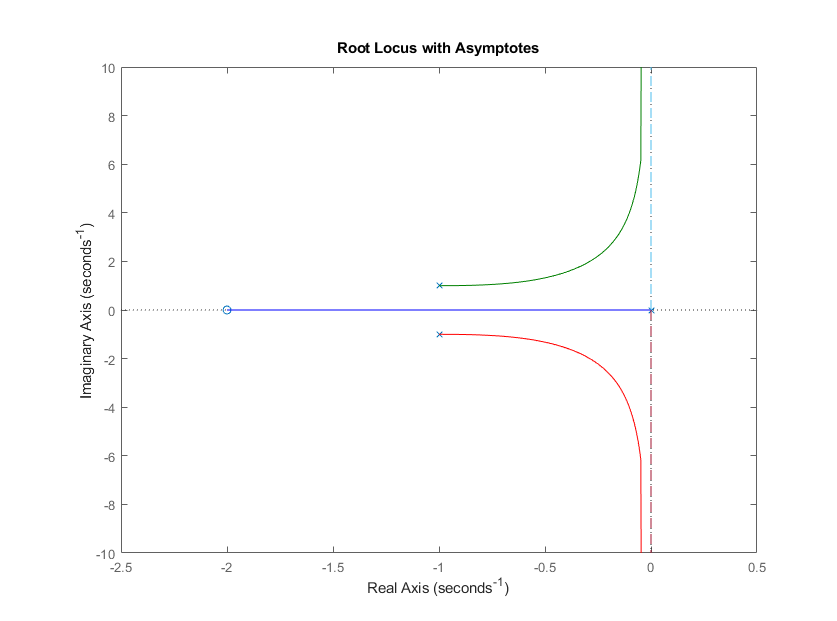
\includegraphics[width=0.8\textwidth]{7-12C_fig.png}

% MATLAB code listing
\begin{lstlisting}
poles = [0, -1 + 1i, -1 - 1i]; % Poles of the system
zero = -2; % Zero of the system
G = zpk(zero, poles, 1); % Transfer function G(s)

figure;
rlocus(G);
hold on;

num_poles = length(poles);
sigma = (sum(real(poles)) - real(zero)) / (num_poles - 1); % Centroid of asymptotes
angles_rad = deg2rad((2*(0:num_poles-2) + 1) * 180 / (num_poles - 1)); % Asymptote angles in degrees

% Plotting asymptotes
for angle = angles_rad
    far_point = sigma + 1000*exp(1i*angle); 
    % Draw the asymptote
    plot([sigma, real(far_point)], [0, imag(far_point)], '--');
end

title('Root Locus with Asymptotes');
xlabel('Real Axis');
ylabel('Imaginary Axis');
hold off;
\end{lstlisting}

\newpage
\subsection*{Solution for Problem part C}

\subsubsection*{Open-Loop Gain \( K(s) \) and its Derivative \( K'(s) \):}
The open-loop transfer function \( K(s) \) for a system with poles at \( 0, -1+j, -1-j \) and no finite zeros is represented as:
\begin{align*}
    K(s) &= \frac{K}{s(s+1-j)(s+1+j)} \\
         &= \frac{K}{s(s^2+2s+2)}.
\end{align*}
\newline
\textbf{Root Locus on Real Axis:} The root locus is found on the real axis to the left of an odd number of poles. Since there are no zeros, the locus extends to the left of all poles.
\newline
\textbf{Breakaway Points:} Breakaway points are identified by differentiating \( K(s) \) and equating it to zero. The derivative is:
\begin{align*}
    K'(s) &= \frac{d}{ds}\left[\frac{K}{s(s^2+2s+2)}\right] \\
          &= \frac{-K(s^2+4s+2)}{s^2(s^2+2s+2)^2}.
\end{align*}
However, solving this for \( s \) does not yield any real roots within the range of the poles, indicating the absence of breakaway points on the real axis.
\newline
\textbf{Asymptotes:}Asymptotes are calculated using:
\begin{align*}
    \sigma &= \frac{\text{Sum of real parts of poles}}{\text{Number of poles - Number of zeros}} = \frac{0+(-1)+(-1)}{3-0} = -\frac{2}{3}, \\
    \phi &= \frac{(2i+1)\pi}{3} = 60^\circ, 180^\circ, 300^\circ \text{ for } i=0,1,2.
\end{align*}
These asymptote angles guide the infinite branches of the root locus.
\newline
\textbf{Departure Angles:} Departure angles are crucial for poles on the complex plane. They are calculated as follows for the pole at \( -1+j \):
\[\angle 1 - (\angle s|_{s=-1+j} + \angle(s+1+j)|_{s=-1+j} + \theta) = 180^\circ\]
With \(\theta_1 = 135^\circ\) and \(\theta_2 = 90^\circ\), we find \(\theta = -45^\circ\).
\newline
\textbf{Intersection with the Imaginary Axis and Stability Analysis:}
The characteristic equation is \( s^3 + 2s^2 + 2s + K = 0 \). Substituting \( s = j\omega \) and separating the real and imaginary parts, we set them to zero:
\begin{align*}
    -\omega^3 + 2\omega &= 0 \implies \omega = 0, \pm \sqrt{2}, \\
    -2\omega^2 + K &= 0 \implies K = 0, 4.
\end{align*}
The system is stable for \( K \in [0, 4) \) and becomes unstable for \( K > 4 \).

% Importing the root locus plot image
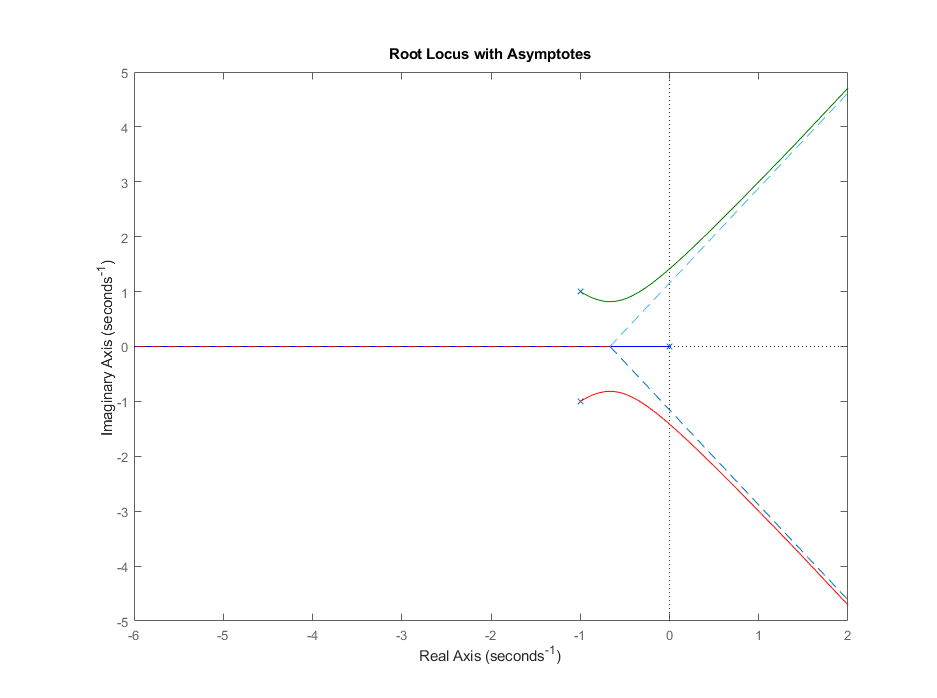
\includegraphics[width=0.8\textwidth]{7-12D_fig.png}

% MATLAB code listing
\begin{lstlisting}
poles = [0, -1 + 1i, -1 - 1i]; % Poles of the system
G = zpk([], poles, 1); % Transfer function G(s)

figure;
rlocus(G);
hold on;

num_poles = length(poles);
sigma = sum(real(poles)) / num_poles; % Centroid of asymptotes
angles_rad = deg2rad((2*(0:num_poles-1) + 1) * 180 / num_poles); % Asymptote angles in degrees

% Plotting asymptotes
for angle = angles_rad
    far_point = sigma + 1000*exp(1i*angle); 
    % Draw the asymptote
    plot([sigma, real(far_point)], [0, imag(far_point)], '--');
end

title('Root Locus with Asymptotes');
xlabel('Real Axis');
ylabel('Imaginary Axis');
hold off;
\end{lstlisting}









\newpage
\section*{Problem 7-16 [30 points]}
Consider a unity-feedback control system with the following forward-path transfer functions:

\begin{enumerate}
    \item \( G(s) = \frac{K}{s(s+2)(s+4)(s+10)} \)
    \item \( G(s) = \frac{K(s^2+4)}{(s+2)^2(s+5)(s+6)} \)
\end{enumerate}

Construct the root loci for \( K \geq 0 \). Determine the value of \( K \) that results in a relative damping ratio of \( 0.707 \) for the closed-loop system, as measured by the dominant complex characteristic equation roots. Verify the answer using MATLAB.
\newpage
\section*{For Transfer Function 1: \( G(s) = \frac{K}{s(s+2)(s+4)(s+10)} \)}

\begin{enumerate}
    \item \textbf{Poles and Zeros:}
    \begin{itemize}
        \item Poles: \( 0, -2, -4, -10 \)
        \item Zeros: None
    \end{itemize}

    \item \textbf{Asymptotes:}
    \begin{itemize}
        \item Number of Asymptotes: \( n - m = 4 - 0 = 4 \) (where \( n \) is number of poles and \( m \) is number of zeros)
        \item Angles of Asymptotes: \( \theta = \frac{(2k+1)180^\circ}{n-m} \) for \( k = 0, 1, 2, 3 \)
        \begin{itemize}
            \item For \( k = 0 \): \( \theta = 45^\circ \)
            \item For \( k = 1 \): \( \theta = 135^\circ \)
            \item For \( k = 2 \): \( \theta = 225^\circ \)
            \item For \( k = 3 \): \( \theta = 315^\circ \)
        \end{itemize}
        \item Intersection with Real Axis: \( \sigma = \frac{\sum \text{poles} - \sum \text{zeros}}{n - m} = \frac{0 - 2 - 4 - 10}{4} = -4 \)
    \end{itemize}

    \item \textbf{Break Away/Break-In Points:}

The characteristic equation is \( 1 + KG(s) = 0 \) or \( s(s+2)(s+4)(s+10) + K = 0 \).

First, rearrange the equation to express \( K \) as a function of \( s \):
\[ K = -s(s+2)(s+4)(s+10) \]

Now, differentiate both sides of this equation with respect to \( s \):
\begin{align*}
\frac{dK}{ds} &= \frac{d}{ds} \left[ -s(s+2)(s+4)(s+10) \right] \\
&= -\left[ (s+2)(s+4)(s+10) + s(s+4)(s+10) + s(s+2)(s+10) + s(s+2)(s+4)\right] \\
&= 4s^3+48s^2+136s+80
\end{align*}


    \item \textbf{Departure and Arrival Angles:}
    \begin{itemize}
        \item Since there are no zeros, there are no arrival angles.
        \item Departure angles are not applicable as all poles are real.
    \end{itemize}
    \item \textbf{Finding angle of damping factor:}
    
In control system analysis, the damping factor \( \zeta \) characterizes a system's transient response. It is defined for a second-order system as:
\[ \zeta = \frac{-\sigma}{\sqrt{\sigma^2 + \omega_n^2}} \]
where \( \sigma \) is the pole's real part, and \( \omega_n \) is the natural frequency.

A damping factor of \( \zeta = \sqrt{2}/2 \) or about \( 0.707 \) signifies a critically damped system, marking the boundary between underdamped and overdamped states. This condition implies that the system's poles in the complex plane form a \( 45^\circ \) angle with the negative real axis. The angle \( \theta \), derived from the pole's position in the s-plane, is calculated as:
\[ \theta = \tan^{-1}\left(\frac{\text{Imaginary part of pole}}{\text{Real part of pole}}\right) = \tan^{-1}(1) = 45^\circ \]

Therefore, a \( 0.707 \) damping factor corresponds to pole angles of \( 45^\circ \) in the s-plane, indicative of a critically damped system.

        
    \item \textbf{Root Locus Plot:}
    \newline
    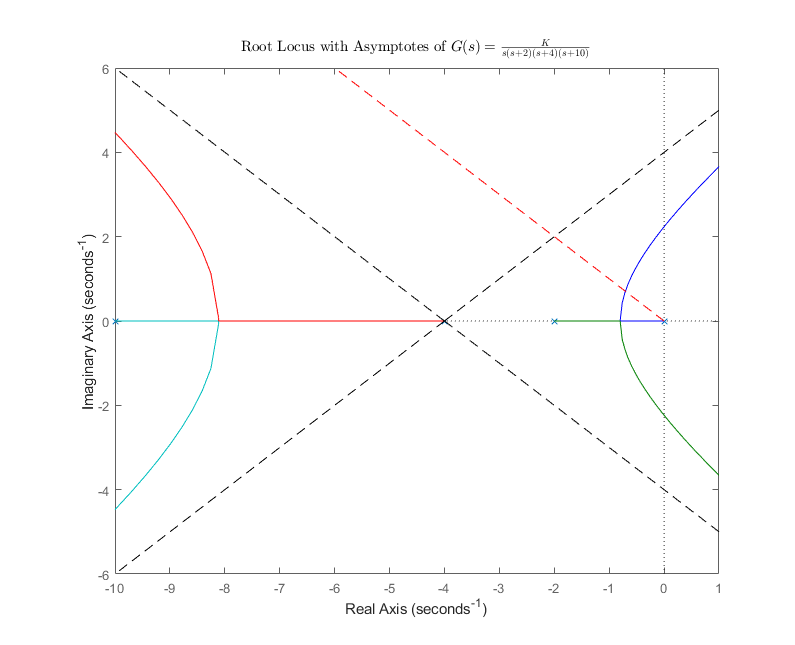
\includegraphics[width=0.9\textwidth]{7-16A.png}
\begin{lstlisting}[caption={MATLAB Code to Plot Root Locus of \( G(s) \)}]
% Define the zeros, poles, and gain of the transfer function
zeros = [];
poles = [0, -2, -4, -10];
gain = 1;

% Create the transfer function
G = zpk(zeros, poles, gain);

% Plot the root locus
figure;
rlocus(G);
hold on;

% Calculate the centroid of the asymptotes
centroid = (sum(poles) - sum(zeros)) / (length(poles) - length(zeros));

% Calculate and plot the asymptotes
n_asymptotes = length(poles) - length(zeros);
for k = 0:n_asymptotes-1
    angle = ((2*k + 1) * pi) / n_asymptotes;
    x = centroid + 1000 * cos(angle);
    y = 1000 * sin(angle);
    plot([centroid, x], [0, y], '--k'); % dashed line for asymptotes
end

% Plot the 135-degree line
angle_135 = 3*pi/4; % 135 degrees in radians
x_135 = 1000 * cos(angle_135);
y_135 = 1000 * sin(angle_135);
plot([0, x_135], [0, y_135], '--r'); % red dashed line for 135-degree angle

% Setting the title and labels
title('Root Locus with Asymptotes of $G(s) = \frac{K}{s(s+2)(s+4)(s+10)}$', 'Interpreter', 'latex');
xlabel('Real Axis');
ylabel('Imaginary Axis');
ylim([-6 6])
xlim([-10 1])
hold off;
\end{lstlisting}
\item \textbf{Finding K:}

Upon visual inspection of the root locus via MATLAB, the intersection of the 45-degree line and the root locus is found to be at \( s = -0.70447 + j0.70447 \). To determine the corresponding gain \( K \) at this intersection point, the characteristic equation of the unity-feedback system is used.

Substituting \( s = -0.70447 + j0.70447 \) into the characteristic equation from earlier yields:
\[ K = -(-0.70447 + j0.70447)\left(-0.70447 + j0.70447 + 2\right)\left(-0.70447 + j0.70447 + 4\right)\left(-0.70447 + j0.70447 + 10\right) \]

The calculation results in a gain \( K \) value of approximately \( 46.155 \), indicating the required gain to achieve the damping factor corresponding to this intersection point.

\end{enumerate}
\newpage

\section*{For Transfer Function 2: \( G(s) = \frac{K(s^2+4)}{(s+2)^2(s+5)(s+6)} \)}

\begin{enumerate}
    \item \textbf{Poles and Zeros:}
    \begin{itemize}
        \item Poles: \( -2, -2, -5, -6 \)
        \item Zeros: \( 2j, -2j \)
    \end{itemize}

    \item \textbf{Asymptotes:}
    \begin{itemize}
        \item Number of Asymptotes: \( n - m = 4 - 2 = 2 \)
        \item Angles of Asymptotes: 
        \begin{itemize}
            \item For \( k = 0 \): \( \theta = 90^\circ \)
            \item For \( k = 1 \): \( \theta = 270^\circ \)
        \end{itemize}
        \item Intersection with Real Axis: \( \sigma = \frac{(-2) \times 2 - 5 - 6}{2} = -7.5 \)
    \end{itemize}

    \item \textbf{Break Away/Break-In Points:}

To find the breakaway points, we need to solve the derivative of the polynomial part of the characteristic equation set to zero:
\[
\frac{d}{ds}\left( \frac{s^2+4}{(s+2)^2(s+5)(s+6)} \right) = 0.
\]

This results in the polynomial:
\[
6s^5 + 75s^4 + 328s^3 + 672s^2 + 864s + 656 = 0.
\]

Solving this derivative, we find the roots are approximately:
\begin{align*}
s_1 &= -2, \\
s_2 &= -5.6, \\
s_3 &= -3.94, \\
s_4 &= -0.48 - 1.5i, \\
s_5 &= -0.48 + 1.5i.
\end{align*}

The last three roots are discarded as they do not lie on the root locus:
\begin{align*}
s &= -2, \\
s &= -5.6.
\end{align*}

These are the potential breakaway points of the system.


    \item \textbf{Departure and Arrival Angles:}
\section*{Arrival Angle Calculation for \( 2j \)}

Given the angles contributed by the poles to the zero at \( 2j \), we have:

\begin{align*}
\angle \theta_1 &= 90^\circ \\
\angle \theta_2 &= 45^\circ \\
\angle \theta_3 &= 21.8^\circ \\
\angle \theta_4 &= 18.4^\circ
\end{align*}

The arrival angle \( \theta \) can be found by subtracting the sum of the angles contributed by the poles from \( 180^\circ \):

\[
\theta = 180^\circ - (\angle \theta_2 + \angle \theta_3 + \angle \theta_4)
\]

Substituting the values, we get:

\[
\theta = 180^\circ - (45^\circ + 21.8^\circ + 18.4^\circ)
\]

\[
\theta = 220^\circ
\]

\end{enumerate}

\section*{Calculations}
For the intersections from MATLAB:

\begin{itemize}
    \item Intersection \#1: \( s = -1.2003 + 1.2003j \)
    \item Intersection \#2: \( s = -6.828 + 6.828j \)
\end{itemize}
\noindent
The calculations are as follows:
For \( s = -1.2003 + 1.2003j \), the value of \( K \) is calculated as:
\[ K = \frac{((-1.2003 + 1.2003j)+2)^2((-1.2003 + 1.2003j)+5)((-1.2003 + 1.2003j)+6)}{((-1.2003 + 1.2003j)^2+4)} \]
\[ K \approx 8.319 \]

For \( s = -6.828 + 6.828j \), the value of \( K \) is calculated as:
\[ K = \frac{((-6.828 + 6.828j)+2)^2((-6.828 + 6.828j)+5)((-6.828 + 6.828j)+6)}{((-6.828 + 6.828j)^2+4)} \]
\[ K \approx 36.429 \]

   \textbf{Root Locus Plot:}
    \newline
    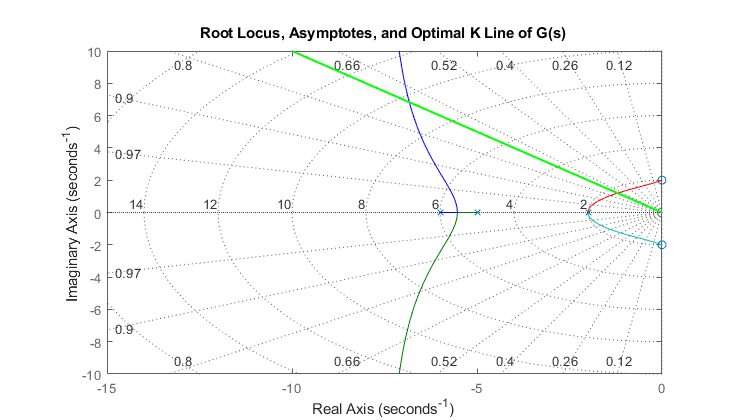
\includegraphics[width=0.9\textwidth]{7-16B.png}
\begin{lstlisting}
% Define the numerator and denominator of the transfer function G(s)
numerator = [1 0 4];
denominator = conv([1 2], conv([1 2], conv([1 5], [1 6]))); % Convolution of the factors to get the denominator polynomial

% Create the transfer function in MATLAB
G_s = tf(numerator, denominator);

% Plot the root locus
figure;
rlocus(G_s);
hold on;

% Asymptote information from earlier analysis
asymptote_angles = [90, 270]; % Degrees
asymptote_real_intercept = -7.5; % Real axis intercept

% Plot the asymptotes
for k = 1:length(asymptote_angles)
    % Convert angle to radians for MATLAB functions
    angle_rad = deg2rad(asymptote_angles(k));
    
    % These are very large numbers to ensure the lines go to the edge of the plot
    asymptote_x = asymptote_real_intercept : 0.1 : asymptote_real_intercept + 1000*cos(angle_rad);
    asymptote_y = 0 + (asymptote_x - asymptote_real_intercept)*tan(angle_rad);
    
    % Plot the asymptote
    plot(asymptote_x, asymptote_y, 'r--', 'LineWidth', 1.5); % Dashed red line
end

% Add the 135 degree line to find optimal K value
optimal_angle = 135; % Degrees
optimal_angle_rad = deg2rad(optimal_angle);

% Plot the 135 degree line
x_line = -10:0.1:0; % Change this range as needed
y_line = tan(optimal_angle_rad) * x_line;
plot(x_line, y_line, 'g-', 'LineWidth', 1.5); % Solid green line

% Set plot limits and labels
xlim([-15, 0]);
ylim([-10, 10]);
xlabel('Real Axis');
ylabel('Imaginary Axis');
title('Root Locus, Asymptotes, and Optimal K Line of G(s)');

% Add grid and hold off the plot
grid on;
hold off;

\end{lstlisting}



\newpage
\section*{Problem 7-18 [25 points]}
A unity-feedback control system has the forward-path transfer functions given in the following. Construct the root locus diagram for \( K \geq 0 \). Find the values of \( K \) at all the breakaway points.
\[ G(s) = \frac{K}{s(s+10)(s+20)} \]

\newpage

\section*{Detailed Solution}

\subsection*{Poles and Zeros}
The given system has poles at \(0\), \(-10\), and \(-20\), with no finite zeros. This is deduced from the transfer function \(G(s) = \frac{K}{s(s+10)(s+20)}\).

\subsection*{Root Locus on Axis}
The root locus exists on the real axis segments \([0, -10]\) and \([-20, -\infty]\). These segments are identified based on the number of poles to the right of each segment on the real axis.

\subsection*{Breakaway Points}
The breakaway points are calculated by finding the roots of the derivative of \(G_1(s) = \frac{1}{s(s+10)(s+20)}\). Setting the derivative \(\frac{dG_1}{ds}\) to zero leads to the quadratic equation \(3s^2 + 60s + 200 = 0\). The solutions to this equation are the breakaway points, which are at \(s = -10 - \frac{10\sqrt{3}}{3}\) and \(s = -10 + \frac{10\sqrt{3}}{3}\).

\subsection*{Asymptotes}
The centroid of the asymptotes, \(\sigma\), is calculated as \(\frac{\sum \text{poles} - \sum \text{zeros}}{\text{number of poles} - \text{number of zeros}} = \frac{-30}{3}\). The angles of the asymptotes, \(\phi\), are given by \(\frac{(2i+1)\pi}{3}\) for \(i = 0, 1, 2\), leading to angles of 60°, 180°, and 300°.

\subsection*{Values of \(\omega\) and \(K\) from the Characteristic Equation}
Substituting \(s = j\omega\) in the characteristic equation \(s^3 + 30s^2 + 200s + K = 0\) and separating real and imaginary parts, we get two equations. The imaginary part \(-\omega^3 + 200\omega = 0\) gives \(\omega\) values as \(0, -10\sqrt{2}, 10\sqrt{2}\). The real part \(-30\omega^2 + K = 0\) is used to calculate \(K\), resulting in \(K = 6000\) when \(\omega = 10\sqrt{2}\).

\subsection*{Values of \(K\) at Breakaway Points}
To find \(K\) at the breakaway points, we substitute the \(s\) values into \(K = \frac{s(s+10)(s+20)}{1}\). For \(s = -10 - \frac{10\sqrt{3}}{3}\), \(K\) is approximately \(384.90\). For \(s = -10 + \frac{10\sqrt{3}}{3}\), \(K\) is approximately \(-384.90\). However, as \(K\) represents gain and must be non-negative, the relevant breakaway point for \(K \geq 0\) is \(s = -10 - \frac{10\sqrt{3}}{3}\) with \(K \approx 384.90\).

\newpage
\section*{Root Locus Plot}
\begin{figure}[h]
    \centering
    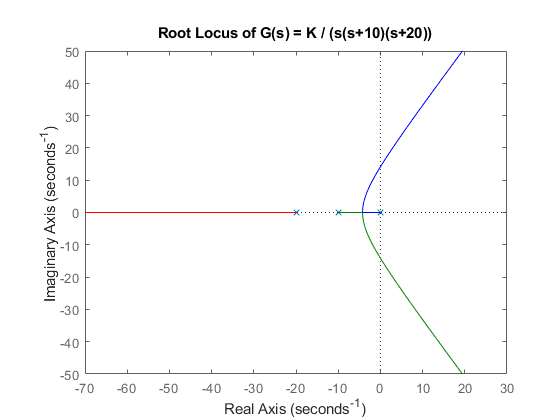
\includegraphics[width=0.8\textwidth]{7-18A.png} % Replace with the actual file name
    \caption{Root Locus Plot of the System}
\end{figure}
\begin{lstlisting}
% Define the numerator and denominator of the transfer function
num = [1];
den = [1 30 200 0];  % Coefficients of s^3 + 30s^2 + 200s + 0

% Create a transfer function model
G = tf(num, den);

% Plot the root locus
rlocus(G);

% Adding title and axis labels
title('Root Locus of G(s) = K / (s(s+10)(s+20))');
xlabel('Real Axis');
ylabel('Imaginary Axis');
\end{lstlisting}



\end{document}
